%!TEX root = main.tex


\subsection{String diagram notation}\label{sec:string_diagrams}

We make use of a string diagram notation for probabilistic reasoning. Graphical models are often employed in causal reasoning, and string diagrams are a kind of graphical notation for representing Markov kernels. The notation comes from the study of Markov categories, which are abstract categories that represent models of the flow of information. For our purposes, we don't use abstract Markov categories but instead focus on the concrete category of Markov kernels on standard measurable sets.

A coherence theorem exists for string diagrams and Markov categories. Applying certain transformations such as planar deformation or any of the commutative comonoid axioms to a string diagram yields an equivalent string diagram. The coherence theorem establishes that any proof constructed using string diagrams in this manner corresponds to a proof in any Markov category \citep{selinger_survey_2011}. More comprehensive introductions to Markov categories can be found in \citet{fritz_synthetic_2020,cho_disintegration_2019}.

\subsection{Products}

On discrete sets, probability measures are vectors and Markov kernels are matrices. Thus given a probability measure $\mu\in \Delta(X)$ and a Markov kernel $\kernel{K}:X\kto Y$, the product $\mu\kernel{K}\in \Delta(Y)$ is a standard vector-matrix product. This idea generalises to measures and Markov kernels in general.

\begin{definition}[measure-kernel product]
Given a probability measure $\mu\in \Delta(X)$ and a Markov kernel $\kernel{K}:X\kto Y$, the product $\mu\kernel{K}\in \Delta(Y)$ is a probability measure such that, for all $A\in \sigalg{Y}$
\begin{align}
     \mu\kernel{K}(A)=\int_{X} \kernel{K}(A|x)\mu(\mathrm{d}x)
\end{align}
\end{definition}

\begin{definition}[kernel-kernel product]
Given Markov kernels $\kernel{K}:X\kto Y$ and $\kernel{L}:Y\kto Z$, the product $\kernel{K}\kernel{L}:X\kto Z$ is a Markov kernel such that, for all $x\in X$ and $B\in \sigalg{Z}$
\begin{align}
     \kernel{K}\kernel{L}(B|x)=\int_{Y} \kernel{L}(B|y)\kernel{K}(\mathrm{d}y|x)
\end{align}
\end{definition}

We can also define a tensor product of kernels.

\begin{definition}[Tensor product of kernels]
Given  $\kernel{K}:X\kto Y$ and $\kernel{M}:W\kto Z$, $\kernel{K}\otimes\kernel{M}:X\times W\kto Y\times Z$ is given by
\begin{align}
    \kernel{K}\otimes\kernel{M}(A\times B|x,w) &= \kernel{K}(A|x)\kernel{M}(B|w)
\end{align}
for all $A\in \sigalg{X}$, $B\in \sigalg{Y}$, $(x,w)\in X\times W$, and this uniquely defines $\kernel{K}\otimes\kernel{M}$.
\end{definition}


\subsection{Elements of string diagrams}

In the string, Markov kernels are drawn as boxes with input and output wires, and probability measures (which are Markov kernels with the domain $\{*\}$) are represented by triangles:

\begin{align}
\kernel{K}&:=\begin{tikzpicture}[baseline={([yshift=-.5ex]current bounding box.center)}]
    \path (0,0) node (A) {}
    ++ (0.5,0) node[kernel] (K) {$\kernel{K}$}
    ++ (0.5,0) node (B) {};
    \draw (A) -- (K) -- (B);
\end{tikzpicture}\\
\mu&:= \begin{tikzpicture}[baseline={([yshift=-.5ex]current bounding box.center)}]
    \path (0,0) node[dist] (K) {$\kernel{P}$}
    ++ (0.5,0) node (B) {};
    \draw (K) -- (B);
\end{tikzpicture}
\end{align}

Given two Markov kernels $\kernel{L}:X\kto Y$ and $\kernel{M}:Y\kto Z$, the product $\kernel{L}\kernel{M}$ is represented by drawing them side by side and joining their wires:

\begin{align}
    \kernel{L}\kernel{M}:= \begin{tikzpicture}[baseline={([yshift=-.5ex]current bounding box.center)}]
    \path (0,0) node (A) {$X$}
    ++ (0.5,0) node[kernel] (K) {$\kernel{K}$}
    ++ (0.7,0) node[kernel] (M) {$\kernel{M}$}
    ++ (0.5,0) node (B) {$Z$};
    \draw (A) -- (K) -- (M) -- (B);
\end{tikzpicture}
\end{align}

Given kernels $\kernel{K}:W\kto Y$ and $\kernel{L}:X\kto Z$, the tensor product $\kernel{K}\otimes\kernel{L}:W\times X\kto Y\times Z$ is graphically represented by drawing kernels in parallel:

\begin{align}
    \kernel{K}\otimes \kernel{L}&:=\begin{tikzpicture}[baseline={([yshift=-.5ex]current bounding box.center)}]
    \path (0,0) node (A) {$W$}
    ++ (0.5,0) node[kernel] (K) {$\kernel{K}$}
    ++ (0.5,0) node (B) {$Y$};
    \path (0,-0.5) node (C) {$X$}
    ++ (0.5,0) node[kernel] (L) {$\kernel{L}$}
    ++ (0.5,0) node (D) {$Z$};
    \draw (A) -- (K) -- (B);
    \draw (C) -- (L) -- (D);
\end{tikzpicture}
\end{align}

We read diagrams from left to right (this is somewhat different to \citet{fritz_synthetic_2020,cho_disintegration_2019,fong_causal_2013} but in line with \citet{selinger_survey_2011}), and any diagram describes a set of nested products and tensor products of Markov kernels. There are a collection of special Markov kernels for which we can replace the generic ``box'' of a Markov kernel with a diagrammatic elements that are visually suggestive of what these kernels accomplish.

The identity map $\text{id}_X:X\kto X$ defined by $(\text{id}_X)(A|x)= \delta_x(A)$ for all $x\in X$, $A\in\sigalg{X}$, is a bare line:

\begin{align}
    \mathrm{id}_X&:=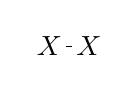
\begin{tikzpicture}[baseline={([yshift=-.5ex]current bounding box.center)}]
    \path (0,0) node (A) {$X$} ++ (0.5,0) node (B) {$X$};
    \draw (A) -- (B);
\end{tikzpicture}
\end{align}

Given some 1-element set $\{*\}$, the erase map $\text{del}_X:X\kto \{*\}$ defined by $(\text{del}_X)(*|x) = 1$ for all $x\in X$ is a Markov kernel that ``discards the input''. It looks like a lit fuse:

\begin{align}
    \text{del}_X&:=\begin{tikzpicture}[baseline={([yshift=-.5ex]current bounding box.center)}]
    \path (0,0) ++ (1,0) node (B) {$X$};
    \draw[-{Rays[n=8]}] (A) -- (B);
\end{tikzpicture}
\end{align}

The copy map $\text{copy}_X:X\kto X\times X$ defined by $(\text{copy}_X)(A\times B|x)=\delta_x(A)\delta_x(B)$ for all $x\in X$, $A,B\in \sigalg{X}$ is a Markov kernel that makes two identical copies of the input. It is drawn as a fork:

\begin{align}
    \text{copy}_X&:=\begin{tikzpicture}[baseline={([yshift=-.5ex]current bounding box.center)}]
    \path (0,0) node (A) {$X$} 
    ++ (0.5,0) node[copymap] (copy0) {}
    ++ (0.5,0.15) node (B) {$X$}
    + (0,-0.3) node (C) {$X$};
    \draw (A) -- (copy0) to [out=45,in=180] (B) (copy0) to [out=-45, in=180] (C);
\end{tikzpicture}
\end{align}

The swap map $\text{swap}_{X,Y}:X\times Y\kto Y\times X$, defined by $(\text{swap}_{X,Y})(A\times B|x,y)=\delta_x(B)\delta_y(A)$ for $(x,y)\in X\times Y$, $A\in \sigalg{X}$ and $B\in \sigalg{Y}$, swaps two inputs and is represented by crossing wires:

\begin{align}
    \text{swap}_{X,Y} &:=  
\begin{tikzpicture}[baseline={([yshift=-.5ex]current bounding box.center)}]
        \path (0,0) node (A) {} 
        + (0,-0.5) node (B) {}
        ++ (1,0) node (C) {}
        + (0,-0.5) node (D) {};
        \draw (A) to [out=0,in=180] (D) (B) to [out=0, in=180] (C);
    \end{tikzpicture}
\end{align}

Diagrams in Markov categories satisfy the commutative comonoid axioms (see Definition \ref{def:mcat})

\begin{align}
    \tikzfig{ccom_lhs} = \tikzfig{ccom_rhs}\label{eq:ccom_1}
\end{align}
\begin{align}
    \tikzfig{ccom2_lhs} = \tikzfig{ccom2_mhs} = \tikzfig{ccom2_rhs}
\end{align}
\begin{align}
    \tikzfig{ccom3_lhs} = \tikzfig{ccom3_rhs}
\end{align}
as well as compatibility with the monoidal structure
\begin{align}
    \tikzfig{mstruct1_lhs} &= \tikzfig{mstruct1_rhs}\\
    \tikzfig{mstruct2_lhs} &= \tikzfig{mstruct2_rhs}
\end{align}
and the naturality of \emph{del}, which means that
\begin{align}
    \tikzfig{naturality_lhs} &= \tikzfig{naturality_rhs}\label{eq:nat}
\end{align}

\subsection{Iterated copy maps and plates}

The previous definitions are standard for Markov categories. We extend the graphical notation with $n$-fold maps and plates, which stand for tensor products repeated $n$ times.

\begin{definition}[$n$-fold copy map]
The $n$-fold copy map $\text{copy}^n_X:X\kto X^n$ is given by
\begin{align}
    \text{copy}^1_X &= \text{copy}_X\\
    \text{copy}^n_X &= \tikzfig{n_fold_copy} &n>1
\end{align}
\end{definition}

In a string diagram, a plate that is annotated $i\in A$ means the tensor product of the $|A|$ elements that appear inside the plate. A wire crossing from outside a plate boundary to the inside of a plate indicates an $|A|$-fold copy map, which we indicate by placing a dot on the plate boundary. We do not define anything that allows wires to cross from the inside of a plate to the outside; wires must terminate within the plate.

Thus, given $\kernel{K}_i:X\kto Y$ for $i\in A$,

\begin{align}
    \bigotimes_{i\in A} \kernel{K}_i &:= \tikzfig{plate_without_copymap}
    \text{copy}^{|A|}_X(\bigotimes_{i\in A} \kernel{K}_i) &:= \tikzfig{plate_with_copymap}
\end{align}


\subsubsection{Examples}
String diagrams can always be converted into definitions involving integrals and tensor products. A number of shortcuts can help to make the translations efficiently.

For arbitrary $\kernel{K}:X\times Y\kto Z$, $\kernel{L}:W\kto Y$

\begin{align}
    \tikzfig{identity_tensor_L} &= (\text{id}_X\otimes \kernel{L})\kernel{K}\\
    [(\text{id}_X\otimes \kernel{L})\kernel{K}](A|x,w) &= \int_{Y}\int_X   \kernel{K}(A|x',y')\kernel{L}(\mathrm{d}y'|w)\delta_x(\mathrm{d}x')\\
                                           &= \int_Y  \kernel{K}(A|x,y') \kernel{L}(dy'|w)
\end{align}

That is, an identity map ``passes its input directly to the next kernel''. 

For arbitrary $\kernel{K}: X\times Y\times Y\kto Z$:

\begin{align}
 \tikzfig{identity_tensor_copy} &= (\text{id}_X\otimes \text{copy}_Y)\kernel{K}\\
 [(\text{id}_X\otimes \text{copy}_Y)\kernel{K}](A|x,y) &= \int_Y\int_Y \kernel{K}(A|x,y',y'') \delta_y(\mathrm{d}y')\delta_y(\mathrm{d}y'')\\
                                           &= \kernel{K}(A|x,y,y)
\end{align}

That is, the copy map ``passes along two copies of its input'' to the next kernel in the product. 

For arbitrary $\kernel{K}:X\times Y\kto Z$

\begin{align}
    \tikzfig{swap_example} &= \text{swap}_{YX} \kernel{K}\\
    (\text{swap}_{YX}\kernel{K})(A|y,x) &= \int_{X\times Y} \kernel{K}(A|x',y')\delta_y(\mathrm{d}y')\delta_x(\mathrm{d}x')\\
                                        &= \kernel{K}(A|x,y)
\end{align}

The swap map before a kernel switches the input arguments.

For arbitrary $\kernel{K}:X\kto Y\times Z$

\begin{align}
    \tikzfig{swap_example_2} &= \kernel{K}\text{swap}_{YZ}\\
    (\kernel{K}\text{swap}_{YZ})(A\times B|x) &= \int_{Y\times Z} \delta_{y}(B)\delta_{z}(A)\kernel{K}(\mathrm{d}y\times\mathrm{d}z|x)\\
    &= \int_{B\times A} \kernel{K}(\mathrm{d}y\times\mathrm{d}z|x)\\
    &= \kernel{K}(B\times A|x)
\end{align}
